\documentclass[tikz,border=14pt]{standalone}
\usepackage{amsmath,amssymb}
\usetikzlibrary{arrows.meta}
\definecolor{ink}{HTML}{E4EDF8}
\definecolor{muted}{HTML}{596B80}
\definecolor{blue}{HTML}{9FC2FF}
\definecolor{teal}{HTML}{63D3BB}
\definecolor{gold}{HTML}{E7C274}
\definecolor{panel}{HTML}{111923}
\pagecolor{panel}
\color{ink}
\begin{document}
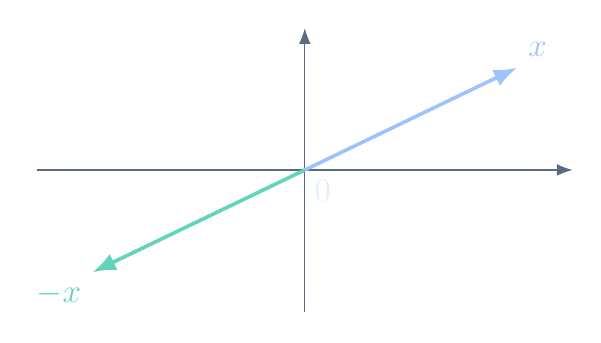
\begin{tikzpicture}[font=\large,text=ink,vec/.style={-{Latex[length=3mm]},line width=1.3pt},axis/.style={muted,-{Latex[length=2mm]},thin}]
\draw[axis] (-3.4,0)--(3.4,0);
\draw[axis] (0,-1.8)--(0,1.8);
\draw[vec,blue] (0,0)--(2.7,1.3) node[above right] {$x$};
\draw[vec,teal] (0,0)--(-2.7,-1.3) node[below left] {$-x$};
\node[below right] at (0,0) {$0$};
\end{tikzpicture}
\end{document}
